\documentclass[a4paper,11pt]{article}

\usepackage[utf8]{inputenc}
\usepackage[margin=1in]{geometry}
\usepackage[T1]{fontenc}
\usepackage{lmodern}
\usepackage{amsmath, amssymb, amsthm}
\usepackage{graphicx}
\usepackage{hyperref}
\usepackage{geometry}
\usepackage{listing}
\usepackage{color}
\setlength{\parindent}{0pt}
\setlength{\parskip}{1em}
\usepackage{booktabs}
\usepackage{caption}
\usepackage[ruled,vlined]{algorithm2e}
\usepackage{subcaption}
\usepackage{bookmark}
\usepackage[
    backend=biber,
    style=authoryear,
  ]{biblatex}


\addbibresource{bibliography.bib}

\title{BART: A Comparison with Non-bayesian Tree Methods}
\author{
    Vincenzo Dorrello 
    \and
    Giulio Frey 
    \and
    Guido Rossetti 
    \and
    Giovanni Scarpato 
}
\date{\today}

\begin{document}

\maketitle

\begin{abstract}
This paper provides a comprehensive comparison between Bayesian Additive Regression Trees (BART) and traditional non-Bayesian tree-based methods for regression problems. We begin by examining the theoretical foundations of decision trees and various ensemble methods, including bagging, random forests, and boosting. We then present BART as a Bayesian nonparametric approach that combines the flexibility of regression trees with the formal uncertainty quantification of Bayesian inference. The paper details BART's probability model, its regularization prior, and the Bayesian backfitting MCMC algorithm used for posterior inference. Through both simulated and real-world data applications, we demonstrate BART's effectiveness in capturing non-linear relationships and compare its predictive performance against other ensemble methods. Using the UCI Abalone dataset, we show that BART achieves superior prediction accuracy compared to random forests, boosting, and bagging when using sufficient numbers of trees, though at a higher computational cost. Our findings suggest that BART's automatic prior-based regularization and ability to quantify uncertainty make it a valuable addition to the tree-based regression toolkit, particularly for complex non-linear modeling tasks.
\end{abstract}

\newpage

\section{Introduction}


The challenge of modeling complex, non-linear relationships in data has led to the development of various tree-based methods in statistical learning. While traditional parametric approaches like linear regression impose strict assumptions on the relationship between predictors and outcomes, tree-based methods offer greater flexibility in capturing non-linear patterns and interaction effects. This paper focuses on comparing Bayesian Additive Regression Trees (BART) with traditional non-Bayesian tree methods, examining their theoretical foundations, implementation approaches, and practical performance.

Tree-based methods have evolved from simple decision trees to sophisticated ensemble approaches such as bagging, random forests, and boosting. These methods combine multiple trees to improve prediction accuracy and reduce overfitting. However, most traditional approaches lack formal uncertainty quantification and require careful tuning of regularization parameters. BART, introduced by \cite{chipmanBARTBayesianAdditive2010}, addresses these limitations by providing a Bayesian framework that automatically handles regularization through prior specifications while offering natural uncertainty estimates.

In our paper, we first provide an overview of the theoretical foundations of decision trees and their ensemble variants. Second, we present a comprehensive analysis of BART's methodology, including its probability model, regularization prior, and the Bayesian backfitting MCMC algorithm used for posterior inference. Third, we demonstrate the practical implementation and performance of these methods through both simulated data and a real-world application using the UCI Abalone dataset.

The paper is organized as follows: Section \ref{decision} introduces decision trees and their fundamental concepts. Section \ref{frequentist} explores frequentist ensemble methods including bagging, random forests, and boosting. Section \ref{bart} provides a detailed examination of BART, including its model specification, prior structure, and posterior sampling approach. Section \ref{Comparison} offers a theoretical comparison of these methods, highlighting their relative strengths and weaknesses. Finally, Section \ref{data_app} presents empirical results from both simulated and real-world data applications, demonstrating the practical implications of choosing between these methods for regression tasks.\footnote{The code repository for this paper is available at this \href{https://github.com/giuliofrey/bart}{link}}


\section{Decision trees}
\label{decision}

Consider a target variable \( Y \) and a \( p \)-dimensional vector of covariates, \( x = (x_1, \ldots, x_p) \). Decision trees are predictive models that make predictions about \( Y \) by partitioning the predictor space—the set of all possible values of \( x \)—into simple, non-overlapping regions. Notice that also linear
regression in a sense partitions the predictor space, but restricts divisions to certain planes. To the contrary, all trees requires is that the partition can be achieved by successive binary splits based on the different predictors. Once we have a partition such as this we base our prediction on the average of the $Y$ in each partition. 

The structure of a decision tree reflects this partitioning process. The tree begins with a root node at the top, representing the entire dataset (or the full covariate space). The root node is split into two subsets according to decision rules based on the predictor variables \( (x_1, \ldots, x_p) \). Each subsequent subset may also be further split into two new subsets, continuing the process recursively. At each split, a new internal node is created, and the segments connecting nodes are called branches. This recursive splitting process, known as \textit{recursive partitioning}, proceeds iteratively until a termination condition is met, such as when further splitting no longer improves predictions or the subsets become too small. The final nodes, called \textit{terminal nodes} or \textit{leaves}, correspond to the smallest subsets created by the tree.

The terminal nodes define a partition of the predictor space into \( J \) non-overlapping regions, \( R_1, R_2, \ldots, R_J \). Each region corresponds to a leaf of the tree. To make a prediction for a given covariate vector \( x \), the tree is traversed starting at the root node. At each internal node, the splitting rule determines whether to proceed to the left or right child node. This process continues until a terminal node is reached. The predicted value \( \hat{y} \) is then assigned based on the region \( x \) belongs to.

When \( Y \) is continuous, the tree is called a \textit{regression tree}, and the predicted value \( \hat{y}_i \) for a new observation \( x_i \) falling into region \( R_j \) is the mean of \( Y \) values for the training observations in \( R_j \). For categorical \( Y \), the tree is referred to as a \textit{classification tree}, and the predicted value is the majority class of \( Y \) among the training observations in \( R_j \). Collectively, these approaches are known as \textit{CART} (Classification and Regression Trees), a term introduced by \cite{Gordon_Breiman_Friedman_Olshen_Stone_1984}.

In this work, we focus specifically on regression trees, which aim to predict a continuous \( Y \) given a training dataset. Regression trees differ fundamentally from linear regression models because they do not impose any parametric form on the relationship between \( x \) and \( Y \). Instead, regression trees use a piecewise constant approximation of this relationship.

To see this, suppose there are \( n \) observations of \( Y \) and \(\mathbf{x} = (x_1, \ldots, x_p) \). The relationship between the covariates and the response variable can be expressed as:
\begin{equation}
Y = f(X) + \epsilon \label{regression}
\end{equation}
where \( \epsilon \) is an error, whose distribution is not necessarily specified. Both regression trees and linear regression models seek to estimate the unknown function \( f(X) \) using the observed data.

The manner in which \( f(X) \) is approximated, however, depends on the model chosen. Linear regression assumes a parametric form:
\[
f(X) = \beta_0 + \sum_{j=1}^p X_j \beta_j,
\]
where \( \beta_0, \beta_1, \ldots, \beta_p \) are coefficients estimated from the data. In contrast, regression trees approximate \( f(X) \) as a stepwise constant function:
\[
f(X) = \sum_{j=1}^J \mu_j \cdot 1(X \in R_j),
\]
where \( R_1, \ldots, R_J \) are the regions defined by the leaves of the tree, and \( \mu_j \) is the mean of \( Y \) for the training observations in region \( R_j \).

The choice between these models depends on the nature of the underlying relationship between the predictor variables and the response variable. If the relationship is approximately linear, a linear regression model is likely to outperform a regression tree. Conversely, if the relationship is highly nonlinear or complex, regression trees can capture such patterns more effectively. Additionally, regression trees have the advantage of being invariant to the scale of the predictor variables, eliminating the need for preprocessing steps like standardization.

This section draws from \cite[Chapter~8]{jamesIntroductionStatisticalLearning2021} and \cite{Genuer_Poggi_2020} to illustrate these concepts.

\subsection{Regression Trees}
A regression tree partitions the \(X\)-space into disjoint regions \(R_j\) and provides a fitted value \(E(Y \mid X \in R_j)\) within each region.
We consider the following notation. Denote by \( T \) the tree structure, consisting of a set of interior node decision rules and a set of $b$ terminal nodes. The decision rules are binary splits of the predictor space of the form \( \{x \in A\} \) vs \( \{x \notin A\} \), where \( A \) is a subset of the range of \( x \). We only consider rules based on the single components of \( x = (x_1, \dots, x_p) \) and of the form \( \{x_i \leq c\} \) vs \( \{x_i > c\} \) for continuous \( x_i \). Let \( M = \{\mu_1, \mu_2, \dots, \mu_b\} \) denote a set of parameter values associated with each of the \( b \) terminal nodes of \( T \). Given the way it is constructed, the tree is a full binary tree, that is, each node has exactly zero or two children. 

We now delve better in the process of building regression trees. As we saw before, they are built in two steps. First, the predictor space (the set of all possible values of the vector of observables $X_1, ...., X_p$) is split into $J$ regions $R_j$ that are distinct and non-overlapping. Secondly, given a new observation $x$ that falls in a region $R_j$, the model predicts the corresponding outcome variable $\hat{y}$ to be the mean of the outcome variables corresponding to the observations in the training set that fall in that same region.



To begin, we have to construct the regions $R_1,..., R_j$. Typically, regions are chosen as $p$-dimensional boxes, where $p$ is the number of regressors. The partition is chosen is such a way to minimize the RSS:  
\begin{equation}
  \{R_1,...,R_J \}=\operatorname*{argmin}_{ \{R_j\}_{j=1}^J}\sum^J_{j=1}\sum_{i\in R_j}\left(y_i-\mu_{R_j}\right)^2
  \label{rss_tree}
\end{equation}
where $\mu_{R_j}$ is the mean of the training observation in the $j$-th box.

It is computationally infeasible to do the optimization problem in \eqref{rss_tree}. Instead of considering all the possible partitions of the predictor space, a top-down, greedy approach, known as recursive binary splitting is used. The approach is \texttt{top-down} since it begins at the top of the tree, and then sequentially splits the predictor space; each split is then indicated by two new branches (hence it is binary). Moreover, the process is \textit{greedy}, since for each step we make the split that generates the greatest reduction of the RSS at that particular step, and we do not choose the best sequence of steps looking ahead.
\\To perform recursive binary splitting, the algorithm considers the set of all predictors $X_1, \ldots, X_p$, and the set of all possible values of the cutpoint $s$, and then choose the predictor $X_j$ and the cutpoint $s$ such that the branching of the tree corresponding to the decision rule:  $$\{X \mid X_j < s\} \quad \text{and} \quad \{X \mid X_j \geq s\}$$ minimizes the RSS. Then, we repeat the process within the resulting subregion, looking again for the predictor and the cutpoint such that the subsequent decision rule minimize the RSS. It is important to note that this time we do not split the entire predictor space but one of the two previously identified regions. This process continues until a stopping condition is reached; the more common requires a minimum number of observation within each splitting nodes.

\subsection{Fitting trees: growing and pruning}

Recursive binary splitting to build a regression tree  is likely to produce good prediction on the training-set but overfit the training data, leading to poor out-of-sample performance.The reason is that the above mentioned procedure is likely to give us a complex tree, which has probably a low bias but high variance in prediction. Indeed, small fluctuations in the training set may lead to different predictions. 

Constraining ex ante the size of trees would be a short-sighted solution, because one could possibly stop too soon, leaving potentially good splits further down in tree unachieved.
\\A better strategy is pruning an already complex tree. This amounts to search for a good intermediate between two extreme cases: a fully developed tree which has high variance but low bias, and a tree consisting of only the root, with high bias but low variance. 
The strategy consists in growing a very large tree $T_0$, and then prune it back in order to obtain a subtree. To do so, we use cost complexity pruning, also know as weakest link pruning.

Consider a sequence of subtrees of $T_0$, $\{T\}_\alpha$ indexed by a non-negative tuning parameter $\alpha$.
For each value of $\alpha$, there is a subtree $T \subset T_0$ such that
$$\sum_{m=1}^{|T|} \sum_{i : x_i \in R_m} \left( y_i - \mu_{R_m} \right)^2 + \alpha |T|$$
is as small as possible, where $|T|$ represents the number of terminal nodes of the tree T, $R_m$ is the subset of the predictor space corresponding to the $m$-th terminal node, $\mu_{R_m}$ is the predicted response associated with $R_m$.
The tuning parameter $\alpha$ controls the trade-off between a sub-tree complexity and and its fit to the training data, the higher the $\alpha$, the more terminal nodes a tree has, the smaller a subtree is.
The value for $\alpha$ can be chosen using a validation set or trough cross-validation.

\subsection{Pros and Cons of decision trees}
Overall, regression trees offer much greater flexibility in handling the relation between covariates and output than linear models do. This comes from the fact that fitting a regression tree amounts to estimate a stepwise relation between $y$ and the covariates $x$ that can proxy well non-linear patterns. They can more naturally incorpo
rate interaction effects. 

Greater flexibility comes in handy also when dealing with missing values. Tree offer an effective way to overcome this issue, by constructing surrogate variables. Exploiting correlation between predictors, they may decrease the effect of missing data. 

So far we considered only binary splits, thus an interesting question would be if a model with more than two splits at each note is a valid idea. However, it turns out that in general is not a good strategy. The issue is that multiple splits fragment the dataset too quickly. Moreover, since multiple splits can be achieved by a series of binary splits, the latter approach is preferred.

The interpretability of trees has been one of the driving forces of its success. Indeed, thanks to their structure, is straightforward to understand why, for a given $x$, we expect a particular value of $y$, following a series of decision rules. Small trees are visually easy to interpret. Moreover, trees build in such a way are a computationally fast method, that easily scales with large datasets.

However, one of the main disadvantages of this setting, is that trees are non-robust. They suffer from high variance: a small change in the data can lead to a large change in the estimation. The main reason of this instability is the hierarchical structure of the process as the effect of an error in one of the first nodes is propagated to the other nodes below it. This is heightened by the fact that single trees tend to overfit, and spurious correlations in the training data can be mistaken as structural patterns and included in the decision rules. This may lead to bad out-of-sample predictive performance. High variance is the main reasons that simple regression trees are generally not used. Instead, ensemble methods are preferred. 

\section{Frequentist ensemble methods}
\label{frequentist}

We highlighted that individual decision trees tend to overfit and to be sensitive to the training data they were built on. To counteract this, ensemble methods were proposed where multiple models
are aggregated or averaged over to give a more stable and
generalisable solution.

In general, ensemble methods combine the fit from many (hundreds, thousands) simpler models to get an overall predictor. 
All the models we are going to discuss, namely Bagging, Boosting, Random Forest and Bayesian Additive Regression Trees are ensemble methods, for which the simpler models consist of regression trees.


\subsection{Bagging}
Bagging, which stands for Bootstrap Aggregation, is a general technique that aims at reducing the variance of a statistical learning method. It is baseed on the fact that, given independent observation, averaging over them reduces variance.


For the case of regression trees, the main problem of using a single tree as a prediction method is that perturbing the learning set can cause significant changes in the predictor constructed. 
We would thus like to be able to take many different training sets from the population, to build a different trees for each training set and then to average the resulting predictions. However this is unfeasible since we do not have access to many training sets. 

Hence, we resort to bootstrap. Bootstrapping consists of taking repeated samples, with replacement, from the single available training set. In such a way, we are able to construct $B$ different bootstrapped training sets. Bagging involves creating multiple $B$ copies of the original training set using hte bootstrap, fitting a separate decision tree to each copy. Then it combines the results from each of the $B$ trees to get an overall prediction.
The single predictions for the target function $f(X)$ for each sample are averaged, as
\begin{equation}
  \label{eq_bagging}
  \hat{f}_{\text{bag}}(x) = \frac{1}{B} \sum_{b=1}^{B} \hat{f}^{*b}(x).
\end{equation}
where $B$ is the number of samples of the bootstrapping procedure.

In bagging the trees are grown big and are not pruned. Therefore, each single tree has high variance and low bias. Averaging these different trees reduce the variance.  Bagging can dramatically reduce the variance of unstable procedures such
as trees, leading to improved prediction. 

The drawback of bagging is that we lose interpretability to improve accuracy. When we bag a large number of trees, we can no longer represent the model with a single tree.

\subsection{Random Forest}
A possible problem with bagging is due to the lack of randomization between trees. Indeed, since trees are separately fitted on the bootstrapped training set, it may happen that they share to great amount the same decision rules. This is the case, for example, if there is very strong predictor in the dataset. If this happens, in the collection of bagged trees a vast majority of the trees will use this strong predictor in the top split and they will all be hihgly correlated among themselves.

Correlation among the trees decrease the effectiveness of averaging, as it does not lead to a large reduction in variance, making the entire bagging algorithm less useful. 

 Random Forests starts from bagging and adds another kind of randomization to reduce correlation among trees. Rather than searching over all the covariate space for each decision rule, as the greedy building of the big trees imposes, in random forests each time we make a split in a tree we randomly sample a subset of $m$ covariates to search over. Therefore, the split is allowed to consider only one of those $m$ predictors. Moreover, at each split is considered a new sample of $m$ predictors. This makes the big trees explore more the space of models.
 
 Usually, we choose $m \approx \sqrt{p}$.
On average, $(p - m)/ = p$ of the splits will not even consider the strong predictor, and so other predictors will have more of a chance. Therefore, we can think of this process as decorrelating the trees, making the average of the resulting trees less variable and hence more reliable.


\subsection{Boosting}

Differently from bagging and random forests, boosting does not involve fitting independent trees from many bootstrap samples and averaging the predictions to reduce variance. Instead, it relies on fitting trees sequentially, that is, using information from previously grown trees. Indeed, trees are not fit to bootstrapped versions of the original datasets, but rather to the residual not explained by the remainder of
the trees. Then, its prediction is added, with a weight, to the prediction of the previous trees. This procedure is iterarated until we express the overall prediction of the boosted trees as trhe weighted average of the prediction of the single trees.
This is shown in algorithm \ref{alg_boosting}. 
\begin{algorithm} [h]
  \caption{Boosting for Regression Trees}
  \label{alg_boosting}
  \SetAlgoLined
  \DontPrintSemicolon
  \SetKwInOut{Input}{Input}\SetKwInOut{Output}{Output}
  
  Set $\hat{f}(x) = 0$ and $r_i = y_i$ for all $i$ in the training set.\;
  \For{$b = 1, 2, \ldots, B$}{
      (a) Fit a tree $f^b$ with $d$ splits ($d+1$ terminal nodes) to the training data $(X, r)$.\;
      (b) Update $\hat{f}$ by adding in a shrunken version of the new tree:
      \begin{equation}
      \hat{f}(x) \gets \hat{f}(x) + \lambda f^b(x).
      \end{equation}\;
      (c) Update the residuals:
      \begin{equation}
      r_i \gets r_i - \lambda f^b(x_i).
      \end{equation}\;
  }
  Output the boosted model:
  \begin{equation}
  \hat{f}(x) = \sum_{b=1}^B \lambda f^b(x).
  \end{equation}\;
  
\end{algorithm}

By fitting sequentially new trees on the residual of the previous tree, boosting improves at each iteration the fit marginally. The parameter $d$, which determines the number of terminal nodes, andh the parameter $\lambda$, which weights the contirbution of each tree to the overall prediction, constraint the single trees to be weak learners. By  fitting small trees to the residuals, we slowly improve $\hat{f}$ in areas where it
does not perform well. It is important to mention that in boosting, unlike in bagging, the construction of each tree strongly depends on the trees that have already grown.

The model accounts for three different tuning parameters. The number of of trees $B$, chosen trough cross-validation.  Interestingly, unlike bagging and random forests, boosting can suffer of overfitting if $B$ is too large, since tree are strongly dependent from each other. 
The shrinkage parameter $\lambda$, a small positive number. Common values for $\lambda$ are 0.01 or 0.001, depending on the problem at hand. However, very small values of $\lambda$ often require a very large B to achieve good performances. Lastly, $d$ represents the number of splits in each tree. Often $d=1$ works well. However in this case the tree is called stump since it contains only a single split.

\section{Bayesian additive regression trees}
\label{bart}

The idea for Bayesian Additive Regression Trees (BART) was first developed by Chipman, George, McCulloch (2010 AOAS). Like other ensemble methods (bagging, boosting, random forest), to solve this regression problem \eqref{regression}, BART approximates \( f(x) = \mathbb{E}(y \mid x) \) by a sum of regression trees. 
However, being a Bayesian method, BART requires specifying a full probability model for the data, composed by a likelihood and a prior. 
The likelihood is obtained by assuming normality of the error in the regression \eqref{regression}. In other words, BART assumes 
\begin{equation}
Y = f(X) + \epsilon, \quad \epsilon \sim \mathcal{N}(0, \sigma^2), \label{regression}
\end{equation}
where \( \sigma \) is a parameter.

The function $f$ is modeled with a sum of $m$ regression trees, which are the remaining parameters of the model. As before, we separate the parameter space into the tree structure $T$, which consists of all the decision rules, and $M$, which is the set of leaves or terminal nodes. Leaves are going to be denoted by $\mu$, as they are simply means in a  regression setting.

Thus, in BART the relationship between $(y, X)$ is modeled as: 
\begin{equation}
y = \sum_{j=1}^m g(x; T_j, M_j) + \epsilon, \quad \epsilon \sim N(0, \sigma^2) \label{firstlikelihood}
\end{equation}
where for each binary regression tree \( T_j \) and its associated terminal nodes  \( M_j \), \( g(x; T_j, M_j) \) is the function assigning \( \mu_{ij} \in M_j \)  to \( x \), and \( \mu_{ij} \in M_j \) will be the predicted value of $y$ for $x$. 

 The BART model is completed by a prior on the parameters $ (\{T_j, M_j \}_{j=1}^m, \sigma)$, 
\[
p((T_1, M_1), (T_2, M_2), \ldots, (T_m, M_m), \sigma).
\]
The essential idea of BART is to exploit this prior to keep the individual tree effects in the fit small and avoid overfitting. Indeed, while the number $m$ of trees is fixed, the overall number of parameters (that is the depth of each trees and the number of terminal nodes) is left unspecified. This should make BART prone to overfit the data by growing large and complex trees. To overcome this problem, BART uses a regularization prior, that is a prior set in a way to shrink the model towards simplicity. As an effect of shrinkage, each tree is forced to explain only a limited subset of the relationships between the covariates and the predictor variable. This is similar to what boosting does, with the difference that in boosting, being a frequentist method, shrinkage is regulated by a parameter $\lambda$, which needs tuning. 

Since the space of parameters $ (\{T_j, M_j \}_{j=1}^m, \sigma)$ is high and random dimensional (remember that only the number of trees is specified, but not the numbers of decision rules or of leaves), BART uses Markov Chain Monte Carlo (MCMC) to get draws from posterior distribution.  At every iteration of the MCMC, the software generates a representation of $f$ and a value for $\sigma$ given the data. A single posterior mean estimate of \( f(x) = \mathbb{E}(Y \mid x) \) at any input value $x$ is obtained by a simple average of these successive draws evaluated at \( x \). Further, pointwise uncertainty intervals for \( f(x) \) are easily obtained from the corresponding quantiles of the sample of draws.

Overall, BART can be viewed as a Bayesian nonparametric approach (each tree has unknown size) that fits a parameter-rich model like \eqref{firstlikelihood} using a regularization prior to avoid overfitting. We are going to examine the a sum-of-trees model and implied likelihood first, and then look at the regularization prior.


\subsection{A Sum-of-Trees Model}
As before, and for technical reasons that will be clear in the posterior sampling, BART models each tree separating it into $T$ and $M$. We denote by \( T \) the binary tree structure —the various binary split decision rules of the form \( \{x_q < c\} \) versus \( \{x_q \geq c\} \), with \( c \in \mathbb{R} \) and $x_q$ an element of the vector of covariates $x$. The vector of parameters associated with \( T \), i.e., the collection of terminal node parameters, is denoted by \( M = \{\mu_1, \ldots, \mu_b\} \), where \( b \) is the number of terminal nodes. The $(T, M)$ are to be thought about as a parameter $\theta$ in prior specification and posterior sampling. 

We define a regression tree as a function \( g(x; T, M) \) that assigns the conditional mean \( \mathbb{E}[y \mid x] \) to the parameter \( \mu_i \in M \), i.e., \( \mu_i = g(x; T, M) \rightarrow \mathbb{E}[y \mid x] \) via binary decision rules denoted as \( T \). With this notation, the sum-of-trees model can be more explicitly expressed as
\begin{equation}
Y = \sum_{j=1}^m g(x; T_j, M_j) + \epsilon, \quad \epsilon \sim N(0, \sigma^2) \label{likelihood}
\end{equation}
where for each binary regression tree \( T_j \) and its associated terminal node parameters \( M_j \), \( g(x; T_j, M_j) \) is the function which assigns \( \mu_{j} \in M_j \) to \( x \). Under \eqref{likelihood}, \( \mathbb{E}(Y \mid x) \) equals the sum of all the terminal node \( \mu_{j} \)'s assigned by the $m$ \( g(x \mid T_j, M_j) \)'s.

 As all others sum-of-tree models, the quantity that is being summed and eventually allocated to \( \mathbb{E}(y \mid x) \) is not the regression tree or tree structure, but the value that each \( j \)th tree structure assigns to the subject, that is \( \mu_{j} \). This makes single regression tree is a simple stepwise function, and summing trees amounts to summing together these stepwise functions. As a result, the resulting function $f(x)$  can approximate the nonlinearities and  interactions effects between the covariates $x$.


Given \eqref{likelihood},  the likelihood for a single training instance is:
\[
p(y \mid T_j, M_j, \sigma^2, x) = \mathcal{N}\left(y \mid \sum_{j=1}^{m} g(x; T_j, M_j), \sigma^2\right),
\]
and the likelihood for the entire training dataset (note that $Y = (y_1, \ldots, y_n)$) is:
\[
p(Y \mid T_j, M_j, \sigma^2, X) = \prod_{i=1}^{N} \mathcal{N}\left(y_i \mid \sum_{j=1}^{m} g(x_i; T_j, M_j), \sigma^2\right).
\]

Consider the parameter space $(\{T_j, M_j\}_{j=1}^m, \sigma)$ of model \eqref{likelihood}. The only identified parameter is $\sigma$, because it's the only one that can be estimated as the variance of the residulas. For the trees, only their number $m$ is fixed, while the individual trees remain unidentified and interchangeable. Indeed, the dimension of each tree (namely the number of internal and terminal nodes) is left unbounded. If data demands it, the trees can grow complex, with many leaves and nodes, but they can also remain simple. Moreover, trees can always be swapped one with the other, so they are fundamentally interchangeable. As a result, the only interpretable parameter is $\sigma$-

For this reason, BART can be defined as a nonparametric Bayes approach: since the dimension of $T$ and $M$ is left unbounded, the model does not have a fixed number of parameters. The dimension of each tree is going to be inferred from the data. This high-dimensional and random structure underpins BART's ability to model complex data flexibly and effectively.This interchangeability means the trees themselves lack direct interpretability. Despite the large number of parameters, BART avoids overfitting through the use of an appropriate regularization prior.

\subsection{A regularization prior}

Since each tree \( g(x; T_j, M_j) \) in \eqref{likelihood}, including the variables to split on, the splitting values, and the mean parameters at each terminal node, is unknown, a prior distribution 
\[
p((T_1, M_1), (T_2, M_2), \ldots, (T_m, M_m), \sigma)
\]
over all the parameters of the sum-of-trees model is needed. 

Since the parameter space is high and random dimensional, to avoid overfitting the prior must be chosen in order to keep the contribution of each \(g(x; T_j, M_j)\) small. The prior is thus a regularization prior, that shrinks the model towards simplicity. But there is also a connection to boosting: indeed, the prior ensures that each tree in the ensemble acts as a weak learner. Rather than attempting to fit the overall pattern in the data, each tree focuses on capturing the residual pattern that other trees did not capture. 

\subsubsection{Prior independence and Symmetry}
In order to simplify the specification of the regularization prior, Chipman assumes that  the trees \( \{(T_1, M_1), \ldots, (T_m, M_m)\} \) are independent of each other and of  \( \sigma \). Then, the prior distribution can be written, using the same prior for each $(T, M)$ pair, as:

\[
p[(T_1, M_1), \ldots, (T_m, M_m), \sigma] = \left[ \prod_{j=1}^m p(T_j, M_j) \right] \, p(\sigma).
\]
For each  $(T, M)$ pair, the joint prior is represented as a marginal for $T$ and a conditional for $M$ given $T$. The choice of conditioning on $T_j$ is due the fact that the dimension of $M$ is determined by the number of bottom nodes in the tree, so once $T$ is known, $M$ is just a vector. 
\[
= \left[ \prod_{j=1}^m p(M_j \mid T_j) \, p(T_j) \right] \, p(\sigma).
\]
Given $T_j$, let  \( b_j \)  be the number of terminal nodes in the tree \( T_j \). Then \( M_j = \{\mu_1, \mu_2, \ldots, \mu_{b_j}\} \) is the vector of terminal node parameters associated with \( T_j \).  Chipman at al. assume that node parameters \( \mu_{ij} \in M_j\) are iid, that is $\mu_{ij} \overset{\mathrm{iid}}{\sim} p(\mu_j)$ This implies: 
\[
p(M_j \mid T_j) = \prod_{i=1}^{b_j} p(\mu_{ij} \mid T_j)
\]
Thus we can write the prior distribution for \eqref{likelihood} as:
\[
p[(T_1, M_1), \ldots, (T_m, M_m), \sigma]= \left[ \prod_{j=1}^m \left( \prod_{i=1}^{b_j} p(\mu_{ji} \mid T_j) \right) p(T_j) \right] \, p(\sigma).
\]
Under these assumptions, for the BART prior is sufficient to specify \( p(T_j) \), \( p(\mu_{ij} \mid T_j) \), and \( p(\sigma) \) (note that each $p$ here denote a different probability distribution depending on its input). The idea of regularization prior is to choose them so to have each $T$ small, each $\mu$ small,  and an appropriate $\sigma$  (e.g. smaller than the least squares estimate). 

\subsubsection{The $T_j$ prior}
 Instead of a probability distribution, Chipman specifies a process that can be used to draw a tree from the prior. The \( T_j \) prior, \( p(T_j) \), is specified by three aspects:
\begin{enumerate}
    \item The probability that a node at depth \( d = (0, 1, 2, \ldots) \) is nonterminal is given by:
    \[
    \frac{\alpha}{(1 + d)^\beta}  \quad \text{with} \quad \alpha \in (0, 1) \quad \text{and} \quad \beta \in [0, \infty),
    \]
    where node depth $d$ is defined as the distance from the root. In default \texttt{wbart}, $\alpha$ is set 0.95 and $\beta$ is set equal to 2. As the tree grows and the depth increases, the probability of splitting decreases. This shrinkage mechanism prevents the tree from growing indefinitely. Nonetheless, trees with many terminal nodes can be grown if the data demands it.
    \item The distribution used to select the covariate to split upon in an internal node.This is the uniform prior on available variables in vector $x$.
    \item The distribution used to select the cutoff point in an internal node conditional on the covariate selected. In \texttt{wbart}, this is the uniform prior on the discrete set of available splitting values $c$.
\end{enumerate}

\subsubsection{The \( \mu_{i,j} | T_j \) Prior}
$\mu_{ij} | T_j$ are assumed to be iid. The prior specification for the leaves is $$ \mu_{ji} |T_j \overset{\text{iid}}{\sim}N(\mu_\mu, \sigma_\mu^2)$$
To specify the hyperparameters $\mu_\mu, \sigma_\mu$, \cite{chipmanBARTBayesianAdditive2010} turn to empirical Bayes, that is they  calibrate the prior using the observed variation in \( y \). In particular, note that under equation \eqref{likelihood}, each $y_i$ is the sum of an error $\varepsilon_i$ and $m$ $\mu_{ij}$. Thus, given $\mu_{ij} \mid T_j \sim N(\mu_\mu, \sigma^2_\mu)$, the induced prior on $E(Y \mid x)$ is \(N(m\mu_\mu, \sigma^2_\mu)\). Since we expect that \(\mathbb{E}(Y \mid x)\) lies between \(y_{\text{min}}\) and \(y_{\text{max}}\), we choose \(\mu_\mu\) and \(\sigma_\mu\) such that the induced prior distribution of $E(Y \mid x)$ assigns substantial probability to the interval \((y_{\text{min}}, y_{\text{max}})\). 

To choose $\mu_\mu$, \( y \) is centered around zero by subtracting its sample meand and it is rescaled so that the observed transformed values range from \( y_{\text{min}} = -0.5 \) to \( y_{\text{max}} = 0.5 \). Then the prior we can choose for $\mu_{ij}$ is zero.
On the other hand, $\sigma_\mu$ is picked such that
\[
\sigma_\mu k\sqrt{m} = 0.5.
\]
for some suitable value of $k$ (generally $k=2$).


As \(k\) and/or \(m\) (the number of trees) increase, such a prior shrinks the tree leaves \(\mu_{ij}\) toward zero, limiting the influence of individual tree components and thus making it a weak learner. 

\subsubsection{The \( \sigma \) Prior}
For the prior of the variance of the idiosyncratic error $\varepsilon$ in \eqref{likelihood}, the inverse chi-square distribution is used:
\[
\sigma^2 \sim \frac{\nu \lambda}{\chi^2_\nu} 
\]
We use the the inverse chi-square because it is a conjugate prior for the variance of the normal distribution, and the distribution of the errors $\varepsilon$ in \eqref{likelihood} is assumed to be normal in our probability model: this will make the draw of $\sigma$ from the posterior easy.

The hyperparameters we need to choose are the degrees of freedom $\nu$ and the scale parameter $\lambda$. Again, an empirical Bayesian approach is adopted to assign 
substantial probability to the entire region of plausible values of $\sigma$. The estimate $\hat{\sigma}$ produced by the software \texttt{wbart} we use in our simulation can be either the sample standard deviation of \( y \) (if the number of covariates is more of the numebr of observations), or the residual standard deviation from a least squares linear regression of \( y \) on the original \( X \). 
The value of \( \nu \) is then picked between 3 and 10 to get an appropriate shape of the distribution of $\sigma$, while the value of \( \lambda \) is chosen so that \( p(\sigma < \hat{\sigma}) = q \), where $q = 0.75, 0.95, 0.99$.

\subsection{ Posterior sampling}
Given the observed data \( y \), our Bayesian setup induces a posterior distribution:
\[
\begin{aligned}
p\left( \{T_j, M_j\}_{j=1}^m, \sigma^2 \mid Y, X \right) &\propto p\left( Y \mid \{T_j, M_j\}_{j=1}^m, \sigma^2, X \right) \times p\left( \{T_j, M_j\}_{j=1}^m, \sigma \right)
\end{aligned}
\]
Since the parameter space is highly dimensional, exact calculation of the posterior is infeasible. However, a MCMC algorithm can be used to sample from this posterior. The algorithm allows to obtain a dependent sample from the posterior
 distribution over the space of sum-of-trees models. 

This algorithm is a Gibbs sampler, in which one parameter is drawn from the full conditional, and then you cycle through the others. In particular, the draw of all parameters from the posterior can be simplified into two major draws from full conditionals: first $m$ successive draws of the trees, and then a final draw for $\sigma$.

For notational convenience, let \( T_{(-j)} \) be the set of all trees except \( T_j \), and similarly define \( M_{(-j)} \). Thus, \( T_{(-j)} \) will be a set of \( m - 1 \) trees, and the associated terminal node parameters. 
The Gibbs sampler loops through the trees, sampling:
\begin{enumerate}
    \item  first,  \( m \) successive draws of \( (T_j, M_j) \) conditionally on \( (T_{(-j)}, M_{(-j)}, \sigma^2, y) \):
\begin{equation}
p(T_j, M_j \mid T_{(-j)}, M_{(-j)}, \sigma^2, y), \quad j = 1, \ldots, m, \label{priortree}
\end{equation}
\item then,  draw of \( \sigma^2 \) from the full conditional:
\begin{equation}
p\left(\sigma^2 \mid\{T_j, M_j\}_{j=1}^m, y\right). \label{priorsigma}
\end{equation}
\end{enumerate}
The draw of $\sigma$ from \eqref{priorsigma} is made easy by the choice of a conjugate prior. Indeed, if all the tree models $(T_i, M_i)$ are known, then the function $f$ is known, and we can compute $y$ minus$ f(x)$ to get the residuals of \eqref{firstlikelihood}. Since hte residulas are assumed to be distributed normally, and the inverse chi-squared distribution is (conditionally) the conjugate prior for the variance of the normal distribution, the draw of \( \sigma^2 \) from the posterior is simply a draw from an inverse chi-squared distribution with updated parameters. 
To get the \( m \) draws of the tree models \( (T_j, M_j) \) from \eqref{priortree}, we take advantage of the following reductions. First, observe that the full conditional:
\[
p\left(T_j, M_j \mid T_{(-j)}, M_{(-j)}, \sigma^2, y\right)
\]
depends on \( (T_{(-j)}, M_{(-j)}, y) \) only through:
\begin{equation}
R_j = y - \sum_{k \neq j} g(x; T_k, M_k), \label{residual}
\end{equation}
which for each $j$ is the $n$-vector of residuals of the $m-1$ regression sum-of-trees excluding the \( j \)-th tree. Thus, the \( m \) draws of \( (T_j, M_j) \) given \( (T_{(-j)}, M_{(-j)}, \sigma^2, y) \) are equivalent to \( m \) draws from:
\begin{equation}
p(T_j, M_j \mid R_j, \sigma^2), \quad j = 1, \ldots, m. \label{13}
\end{equation}

Now we use the fact that, by the definition of conditional probability, we can write:
\[
p(T_j, M_j \mid R_j, \sigma^2) = p(M_j \mid T_j, R_j, \sigma^2) \; p(T_j \mid R_j, \sigma^2).
\]
We start from \( p(T_j \mid R_j, \sigma^2) \). Using Bayes' Theorem and standard probability laws, 
\[
p(T_j \mid R_j, \sigma^2) \propto p(T_j) \; p(R_j \mid T_j, \sigma^2) 
\propto p(T_j) \; \int p(R_j, M_j \mid T_j, \sigma^2) \, dM_j.
\]

Expanding further:
\[
p(T_j \mid R_j, \sigma^2) \propto p(T_j) \; \int p(R_j \mid T_j, M_j, \sigma^2) \; p(M_j \mid T_j, \sigma^2) \, dM_j
\]
\[
= p(T_j) \; \int p(R_j \mid T_j, M_j, \sigma^2) \; p(M_j \mid T_j, \sigma^2) \; p(\sigma^2) \, dM_j.
\]

And finally:
\begin{equation}
p(T_j \mid R_j, \sigma^2) \propto p(T_j) \int p(R_j \mid M_j, T_j, \sigma^2) \; p(M_j \mid T_j, \sigma^2) \, dM_j. \label{posterioeT}
\end{equation}

Notice that $R_j$, the $n$-vector of partial residuals, is conditionally normally distributed,and that we have used a conjugate normal prior for $M_j$. Thus, it can easily be integrated it out from \eqref{posterioeT} to obtain $p(T_j \mid R_j, \sigma^2)$ in closed form up to a normalizing constant. Thus we can just draw $T$ alone from \eqref{posterioeT} and then draw $M_j$ conditionally on it.  In other words, the draw from \eqref{13} can be split in two successive steps.
\begin{enumerate}
    \item  first,  we draw  $T_j$ conditional on all the other trees/ on the residula $R_j$ and on $\sigma$ from \eqref{posterioeT}:
\begin{equation}
 T_j \mid R_j, \sigma^2, \label{MH}
\end{equation}
\item then, you draw $M_j$conditional on all the trees and on $\sigma$:
\begin{equation}
M_j \mid T_j, R_j, \sigma^2 \label{drawM}
\end{equation}
\end{enumerate}
The draw of $T_j$ from \eqref{MH} is obtained using a Metropolis-Hastings (MH) algorithm. Let \( T_j^{(i)} \), \( M_j^{(i)} \), and \( \sigma^{(i)} \) denote the values of \( T_j \), \( M_j \), and \( \sigma \) at the \( i \)th MCMC iteration, respectively. Each draw  \( T_j^{(i)} \mid R_j^{(i)}, \sigma^{(i)} \) from \eqref{MH} is obtained using MH. At the MCMC iteration $i$, MH samples $T_j^{(i)}$ by proposing local changes to $T_j^{(i-1)}$. CHanges are either accepted or rejected in such a way that it is still true that the posterior is the stationary distribution. 
The proposal changes to $T_J^{(i-1)}$ that MH can carry are the following: 
\begin{itemize}
    \item \textbf{Grow:} randomly chooses a leaf node and splits it further into left and right children (with probability 0.25). 
    \item \textbf{Prune:} randomly chooses an internal node where both the children are leaf nodes and prunes the two leaf nodes, thereby making the internal node a leaf node (probability 0.25). 
    \item \textbf{Change:} changes the decision rule at a randomly chosen internal node (probbility 0.40)
    \item \textbf{Swap:} swaps the decision rules at a parent-child pair where both the parent and child are internal nodes (probability 0.10)
    \end{itemize}
    Clearly, these moves change the dimension of the tree and thus of the parameter space. The fact that the dimension of the parameter space changes as inference is carried out is indeed a feature of Bayesian nonparametrics. 

Finally, once we have $p(T_j \mid R_j, \sigma^2)$, we are left with the draw $M_j$ from the distribution \eqref{drawM}. Given that the $\mu_{ji}$ are iid, we have: 
$$ p(M_j \mid T_j, R_j, \sigma^2) = \prod_{i=1}^{b_j} p(\mu_{ij} \mid T_j, R_j, \sigma^2),
$$ where the prior on $\mu_{ji}$ is  $N(0, \sigma_\mu^2)$. Notice that, if you call  \( R_{ji} \) the subsets of residuals in the $n$-vector  $R_j$ that are allocated to the terminal node parameter  \( \mu_{ji} \), and call \( n_i \) their number, then \( R_{ji} \mid T_j, \mu_{ji}, \sigma \sim \mathcal{N}(\mu_{ji}, \sigma^2) \). Thus the prior of $\mu_{ji}$ is actually conjugate, and the posterior we are drawing from, $p(\mu_{ji} \mid T_j, \sigma, R_j) \propto p(R_{ji} \mid T_j, \mu_{ji}, \sigma) p(\mu_{ji} \mid T_j)$, is going to be a normal distribution. The draw of \( M_j \) from this normal enables the calculation of the subsequent residual \( R_{j+1} \), which allows the successive draw of \( T_j \). 

The MCMC algorithm is initialized with $m$ simple single node trees, and then iterations are
 repeated until convergence. At each iteration, the dimension of the trees changes. Contrarily to boosting, where trees are fitted sequentially on the residual of the previous, in this algorithm you have a set of trees, and then you cycle through all the trees and keep adjusting one tree, given all the others. For this reason, it is also called Bayesian backfitting. 
The algorithm is summarized in the following figure.
\begin{algorithm} [h]
  \caption{Bayesian backfitting MCMC for posterior inference in BART}
  \label{MCMC}
  \SetAlgoLined
  \DontPrintSemicolon
  \SetKwInOut{Input}{Input}\SetKwInOut{Output}{Output}
  
  \textbf{Inputs:} Training data $(X, Y)$, BART hyperparameters $(\alpha, \beta, m, k, \nu, q)$.\;
  
  \For{$j = 1, \ldots, m$}{ 
      (a) Initialize $T_j^{(0)}$ with a single leaf node.\;
      (b) Sample $M_j^{(0)}$. \tcp*{\textit{$\mu_j = \frac{\overline{Y}}{m}$}}
  }
  
  \For{$i = 1, \ldots, \texttt{maxiter}$}{     
      (c) Sample $\sigma^{(i)} \mid \{T_j^{(i-1)}, M_j^{(i-1)}\}_{j=1}^m$ \tcp*{\textit{Sample from invgamma }}
      
      \For{$j = 1, \ldots, m$}{
          (d) Compute residual $R_j^{(i)}$ \tcp*{\textit{Using \eqref{residual}}}
          
          (e) Sample $T_j^{(i)} \mid R_j^{(i)}, \sigma^{(i)}, T_j^{(i-1)}$ \tcp*{\textit{Using MH}}
          
          (f) Sample $M_j^{(i)} \mid R_j^{(i)}, \sigma^{(i)}, T_j^{(i)}$ \tcp*{\textit{Sample from Gaussian distribution}}
      }
  }
\end{algorithm}
\textit{Adapted from the blog}.

\section{Comparison}
\label{Comparison}

We examined different ensemble methods that combine regression trees to estimate an unknown function $f(X)$ in a regression like 
\[
Y = f(X) + \varepsilon
\]
without assuming linearity.
These ensembles of regression trees allows to model nonlinearity and interaction effects between covariates by fitting some sort of stepwise function on the data. According to Lakshminarayanan (2015), ensembles of regression trees can be
broadly classified into two families: randomized independent regression trees, wherein the trees are grown independently and predictions are averaged to reduce variance, and additive regression trees, wherein each
tree fits the residual not explained by the remainder of
the trees. In the first category there are bagged trees, and random forests, which use use randomization to create a large number of independent trees, and then reduce prediction variance by averaging predictions across the tree \parencite{chipmanBARTBayesianAdditive2010}.

Addititive regression trees methods can be further categorized into those that are fit in a serial fashion, like in boosting, and those fit in an iterative fashion, like
Bayesian additive regression trees (BART). In moth methods, trees are grown dependently one from the other and thus are prone to overfitting and must be regularized. For example, boosting fits a sequence of single trees, using the resedual of the previous tree to fit the subsequent tree. Regularization in boosting is governed by parameters $\lambda$ and $d$, which shrink the contribution of each tree toward zero. In this way, each tree is forced to explain only a part of the overall fit (it is a weak learner). 

On the other hand, BART is a Bayesian method defined by a probability model with a likelihood and a prior. Regularization is performed by the prior distribution, which is set in such a way to prefer simple tree structures $T_j$ and non-extreme predictions at leaves $\mu_{ji}$. The prior thus constrain each tree to be a weak learner, just like in boosting. Since the dimension of the trees (the number of nodes) is left unbounded,  In effect, BART is a nonparametric Bayesian method: the trees are dimensionally adaptive \parencite{chipmanBARTBayesianAdditive2010}.

To fit the sum-of-trees model, BART uses a Bayesian backfitting MCMC algorithm that iteratively constructs and fits successive residuals. Here there is another difference with boosting: while in boosting trees are built sequentially, with each tree explicitly addressing the residual errors of the previous ensemble of trees, in BART a fixed number $m$ of trees is set and trees are adjusted collectively during Markov Chain Monte Carlo (MCMC) iterations to fit the data. In other words, at each MCMC iterations the dimension of the trees is updated.  

Overall, BART's strength comes from the fact that being a Bayesian method its shrinkage parameters does not need tuning, ad the prior will perform shrinkage automatically. In terms of performance, the literature (Chipman et a.) shows that BART has predictive performance comparable to other ensemble methods and far superior to linear regression when nonlinearities are present in the data. 

  
\section{Data Application}
\label{data_app}

We now move to applications of the theoretical insights derived in the previous sections. Firstly, we will focus on simulated data, and then we will cover an application using real word data on Abalones.

\subsection{Simulated data}
We simulate a dataframe with the following generating non-linear function:
\begin{equation}
  y = 2\sin(x)+x+Z \quad Z \sim \mathcal{N}(0,1)
\end{equation}
The dataframe is split in two smaller dataframes to obtain training and testing data.

We first run a single decision tree on the simulated data and we obtain as a result 5 terminal nodes and a 
residual mean deviance of 1.164. 

We now fit a BART model with default parameters:  MCMC have 1100 iterations in total of which 100 are burn-in. We see from figure \ref{plot_sin1} that the BART model is able to fit correctly this non-linear trend.

\begin{figure}
  \centering
  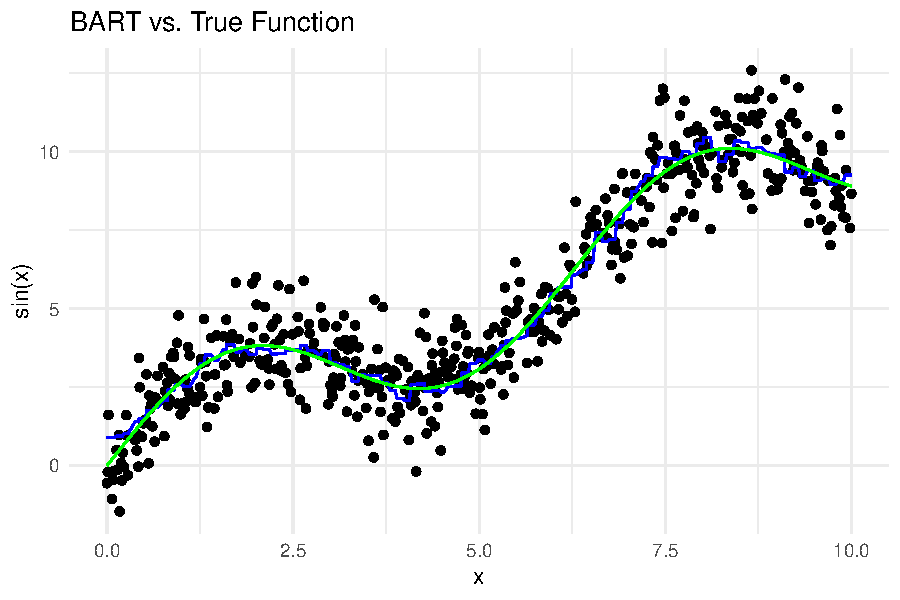
\includegraphics[width=0.7\textwidth]{outputs/sin_plot.pdf}
  \caption{Plot of the estimates (blue) against observations (black) and generating function(green)}
  \label{plot_sin1}
\end{figure}

To check convergence of the posterior, we plot in figure \ref{plot_sin2} the posterior draws of $\sigma$, the uniquely identified parameter. We observe that the MCMC draw converges quickly to the true parameter, although they oscillate with some autocorrelation due to the posterior sampling procedure.

\begin{figure}
  \centering
  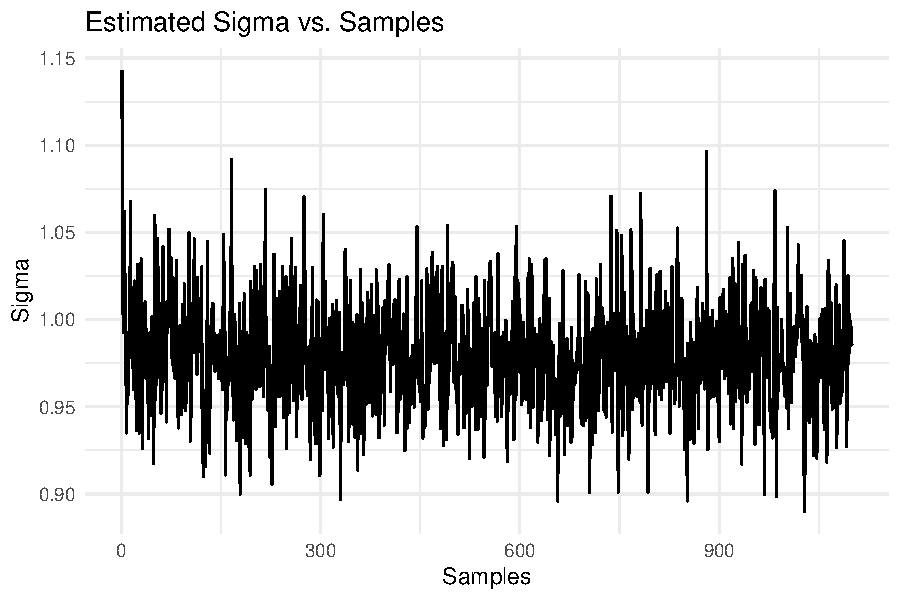
\includegraphics[width=0.7\textwidth]{outputs/sigma_plot.pdf}
  \caption{Value of $\sigma$ over MCMC iterations}
  \label{plot_sin2}
\end{figure}


To check robustness of BART to different prior specifications, we consider different values for the prior mean of $\sigma$,  that are 100, 0.001 and 1 (the true one). With a large $\sigma$, we observe in plot \ref{plot_sin3} underfitting of the data. With a small $\sigma$, holding all the other parameter constant, the regularization prior is still strong enough to avoid the overfitting.

\begin{figure}
  \centering
  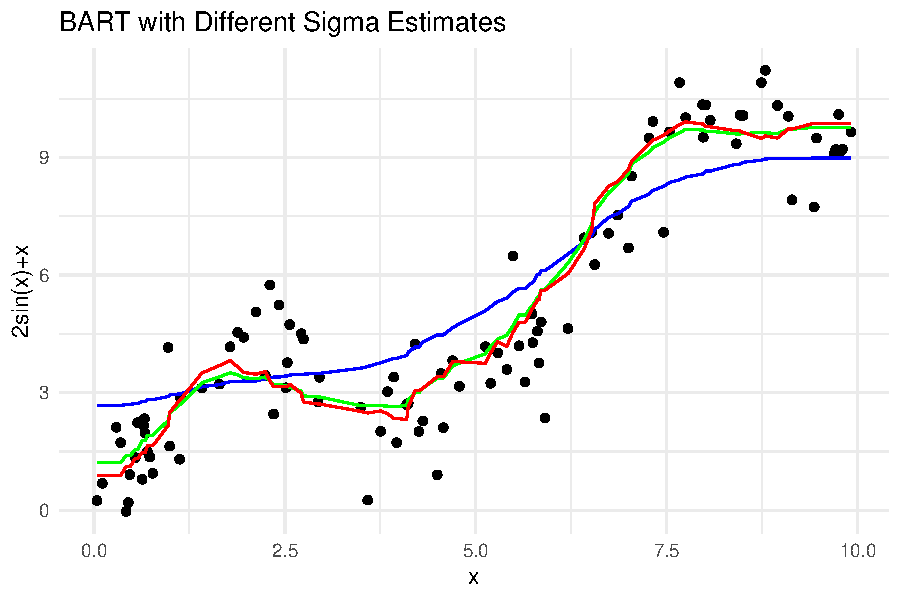
\includegraphics[width=0.7\textwidth]{outputs/sin_plot_diff_sigma.pdf}
  \caption{DIfferent prior mean of $\sigma$}
  \label{plot_sin3}
\end{figure}


\subsection{Predicting the age of an Abalone}

Abalone are marine snails found in various regions around the world. Determining their age is a labor-intensive process, as it requires cutting through the shell, staining it, and then counting the growth rings under a microscope. However, predicting the age of an abalone can also be done by examining other physical characteristics of the individual, which are much easier to assess. This is precisely the motivation behind our application.

We use data abalone characteristics data coming from the UC Irvine Machine Learning Repository \parencite{warwicknashAbalone1994a}, that is described in table \ref{table1}. No data manipulation is necessary, aside from creating a new variable, \( \text{Age} = \text{Rings} + 1.5 \), and removing the column identifying the number of rings.

\begin{table}[]
  \centering
  \begin{tabular}{llllll}

  \toprule
  Variable Name & Role & Type & Description & Units \\
  \midrule
  Sex                  & Feature       & Categorical   & M, F, and I (infant) & -    \\
  Length               & Feature       & Continuous    & Longest shell measurement & mm\\
  Diameter             & Feature       & Continuous    & Perpendicular to length & mm  \\
  Height               & Feature       & Continuous    & With meat in shell      & mm  \\
  Whole\_weight         & Feature       & Continuous    & Whole abalone           & gram\\
  Shucked\_weight       & Feature       & Continuous    & Weight of meat          & gram\\
  Viscera\_weight       & Feature       & Continuous    & Gut weight (after bleeding) & \\
  Shell\_weight         & Feature       & Continuous    & After being dried       & gram\\
  Rings                & Target        & Integer       & +1.5 gives the age in years & - \\

   \bottomrule
  \end{tabular}
  \caption{Table of Variables}
  \label{table1}
  \end{table}

We run BART from \cite{mccullochBARTBayesianAdditive2024}; Boosting from \cite{ridgewayGbmGeneralizedBoosted2024}; Random Forest and Bagging from \cite{breimanRandomForestBreimanCutlers2024}.Our aim is to compare the predictive performance of those methods. In order to do so, we use half of the sample to fit $\hat{y}$, that is the age variable, and half the sample to give us out of bag Mean Squared Errors (MSE) for predicting the same variable. Models are run for various values of T, and for each value, both the mean squared error (MSE) of out-of-sample predictions (shown in plot \ref{plot_mse}) and the computation time (depicted in plot \ref{plot_time}) are recorded.

We observe with a number of trees estimated larger than 500, the BART model is the best performing one, and it reaches also the best performance overall when run with 500 iterations. Although it is the best performer, it is also the model that takes the most to be run, and time of computations scales linearly with the number of trees that are fitted.

\begin{figure}
  \centering
  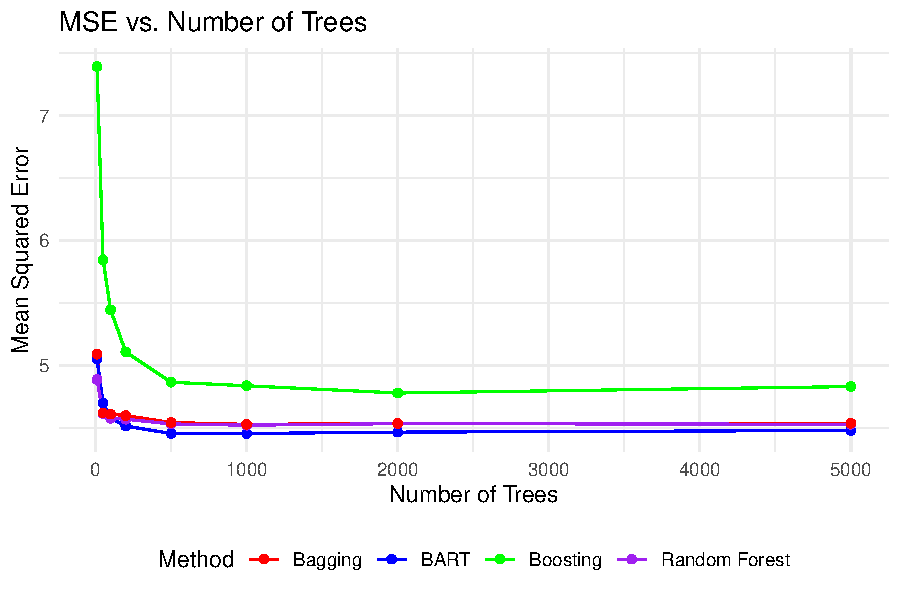
\includegraphics[width=0.7\textwidth]{outputs/mse_plot.pdf}
  \caption{Mean Squared Error for different values of T}
  \label{plot_mse}
\end{figure}

\begin{figure}
  \centering
  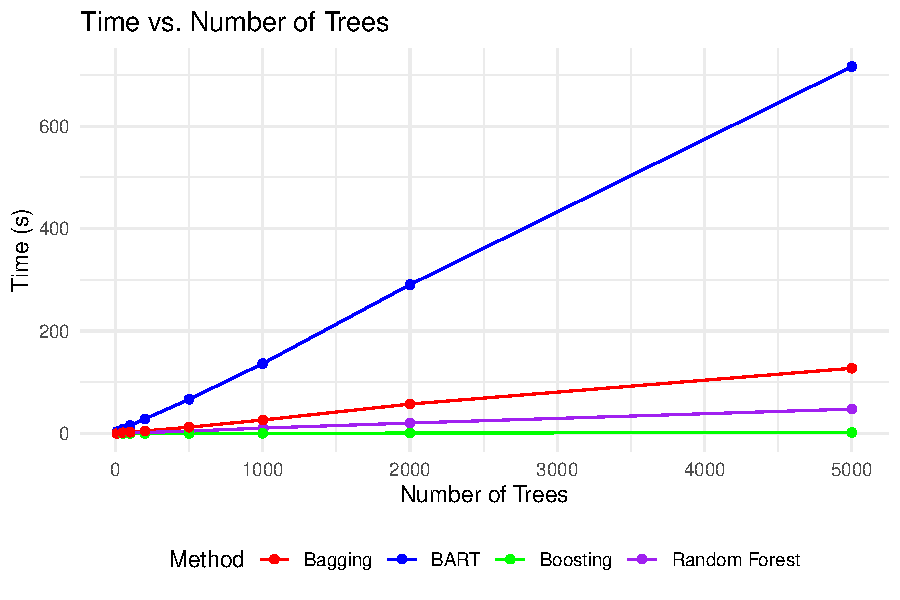
\includegraphics[width=0.7\textwidth]{outputs/time_plot.pdf}
  \caption{Time of computations for different values of T}
  \label{plot_time}
\end{figure}

\begin{table}[ht]
  \centering
  \begin{tabular}{lcc}
  \toprule
  Model           & MSE & Time (s) \\
  \midrule
  BART            & 4.45    & 66.7  \\
  Random Forest   & 4.53    & 4.74  \\
  Boosting        & 4.87    & 0.220 \\
  Bagging         & 4.54    & 12.4  \\
  \bottomrule
  \end{tabular}
  \caption{Model performance with $T=500$}
  \end{table}



\newpage
$ $
\newpage

\printbibliography

\end{document}